\section{Introduction}
\label{sec:intro}
The task of avoiding obstacles is one of the key issues when it comes to the vehicular scenario and it is more difficult to perform it here than it is in static environments.
A vehicle with an obstacle avoidance system is equipped with sensors that measure the distance between the car itself and the obstacle in the same lane. If an autonomous car encounters an obstacle, it is expected to move temporarily to another lane and move back to the original lane once it has driven past the obstacle. This type of control can be implemented using a Model Predictive Control (MPC).
An MPC is an advanced control method that works in discrete time and uses a model of the system to make predictions about the system’s future behavior. MPC solves an online optimization algorithm to find the optimal control action that drives the predicted output to the reference \cite{MPC_Def}.  In other words, from a set of state values, and with respect to a model, it optimizes a problem around an objective and gives a sequence of control signals as outputs. The first set of control values are then used as inputs to the system plant, and after a short period, set as the \emph{system time step}, the new state values are measured and the process is repeated.
The overall objectives of the MPC are:
\begin{itemize}
 

\item prevent that input and output constraints are violated;
\item optimize some input variables, while other outputs are kept in specified ranges,
\item prevent the input variables from having excessive variations.
\end{itemize}
Figure \ref{fig:MPC_Block} shows a block diagram for a Model Predictive Control.
\begin{figure}[H]
    \centering
    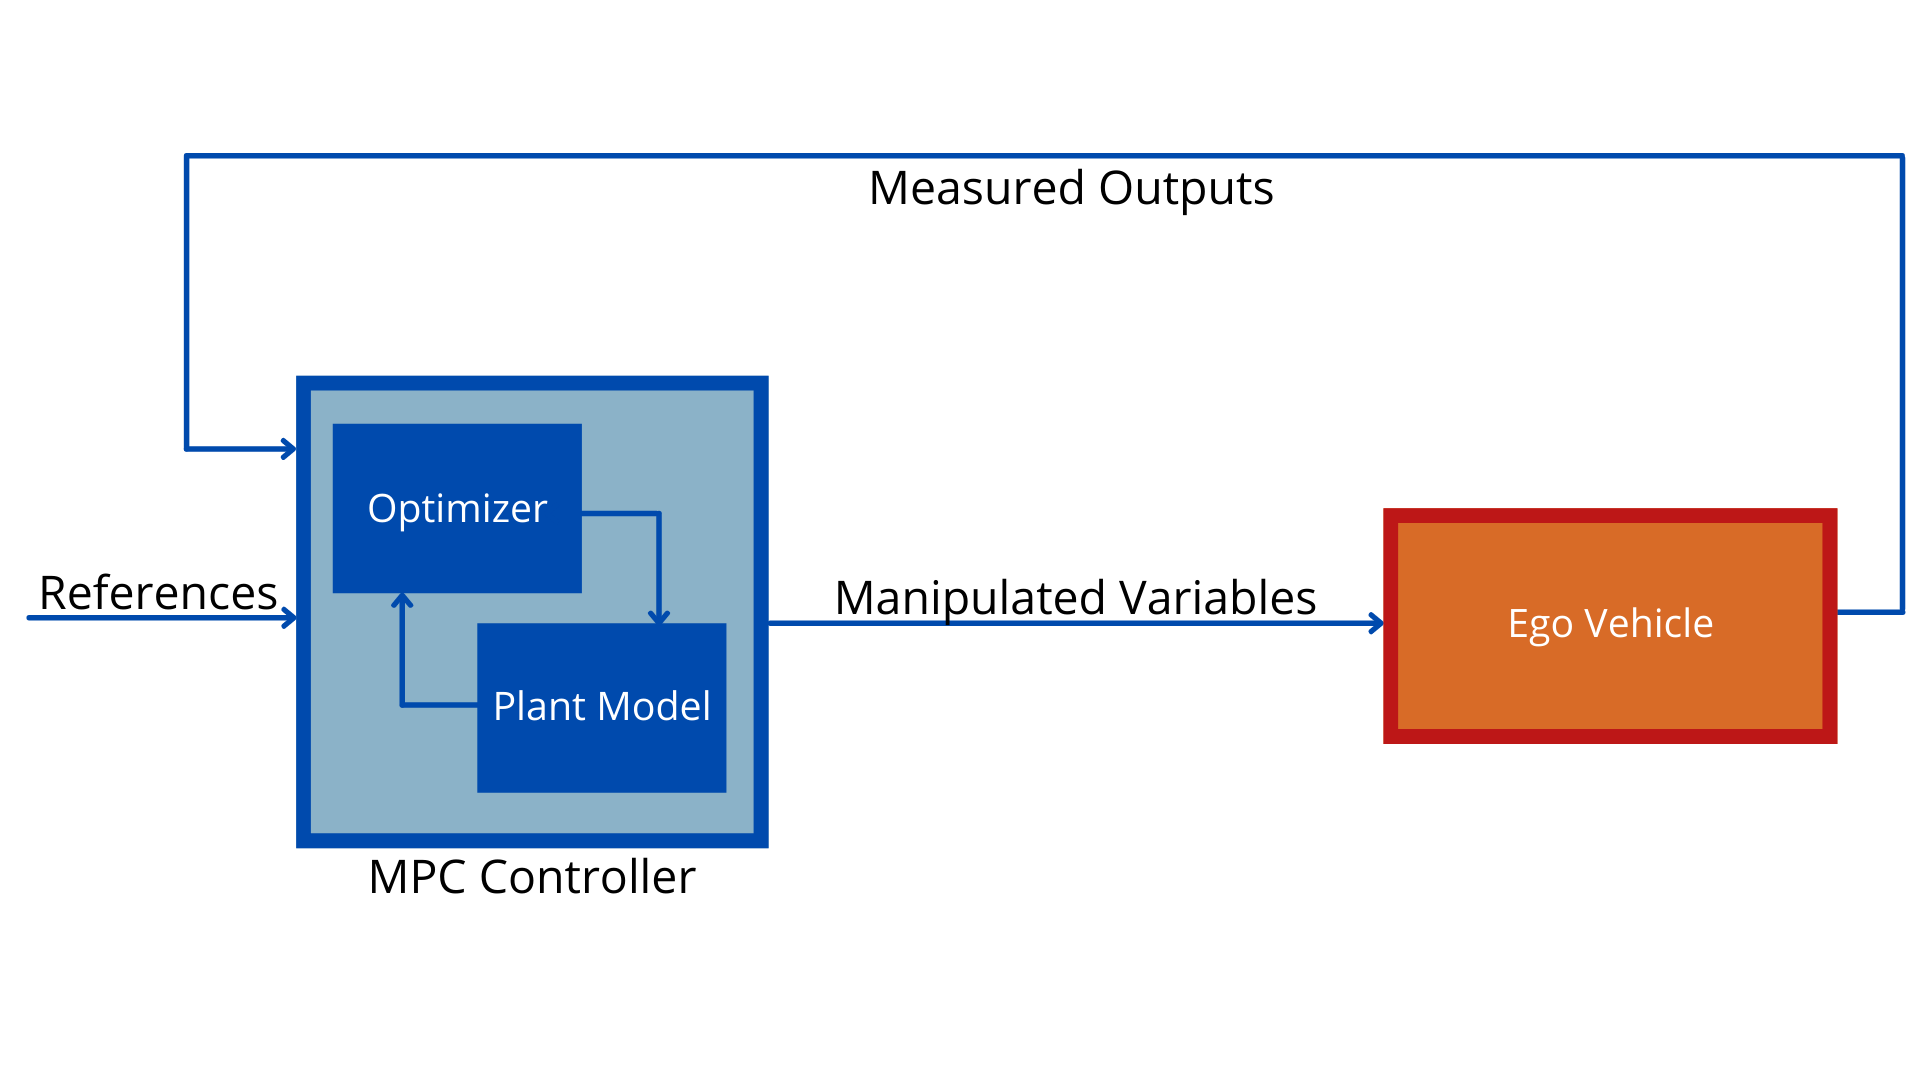
\includegraphics[width=1\textwidth]{Figures/mpcblock.png}
    \caption{MPC Block Diagram}
      \label{fig:MPC_Block}
\end{figure}
An MPC controller has two main functional blocks: the optimizer and the plant model.
The dynamic optimizer allows to find the optimal input that gives the minimum
value of the cost function taking into account all the constraints. Generally, a non linear model is used for the validation of the controller, while the plant model used for the MPC is a linearized version of the actual plant.\\
Our project is based on the use of an \emph{adaptive} MPC which means that the plant state has to be measured again to be adopted as the linearization point for the next step of the predictive control. When the plant state is re-sampled, the whole process
computes again the calculations starting from the new current state.

\subsection{Model-Based Design}
When developing a project, especially concerning embedded systems, it is crucial to follow a process model which illustrates the high-level activities and their phasing during development.\\
As stated in \cite{FOWLER20151} \emph{``Process models provide high-level perspective that helps team members understand what activities to do and what progress  has been made on each of those development activities"}.\\
The development process of our system is based on the V-model shown in Figure \ref{fig:V_model}.
Starting from the general V-model we have tailored our own V-model in order to meet our needs; doing so we have managed to skip some unnecessary steps in the development process while still being compliant with the definition of the V-model itself.

\begin{figure}[H]
    \centering
    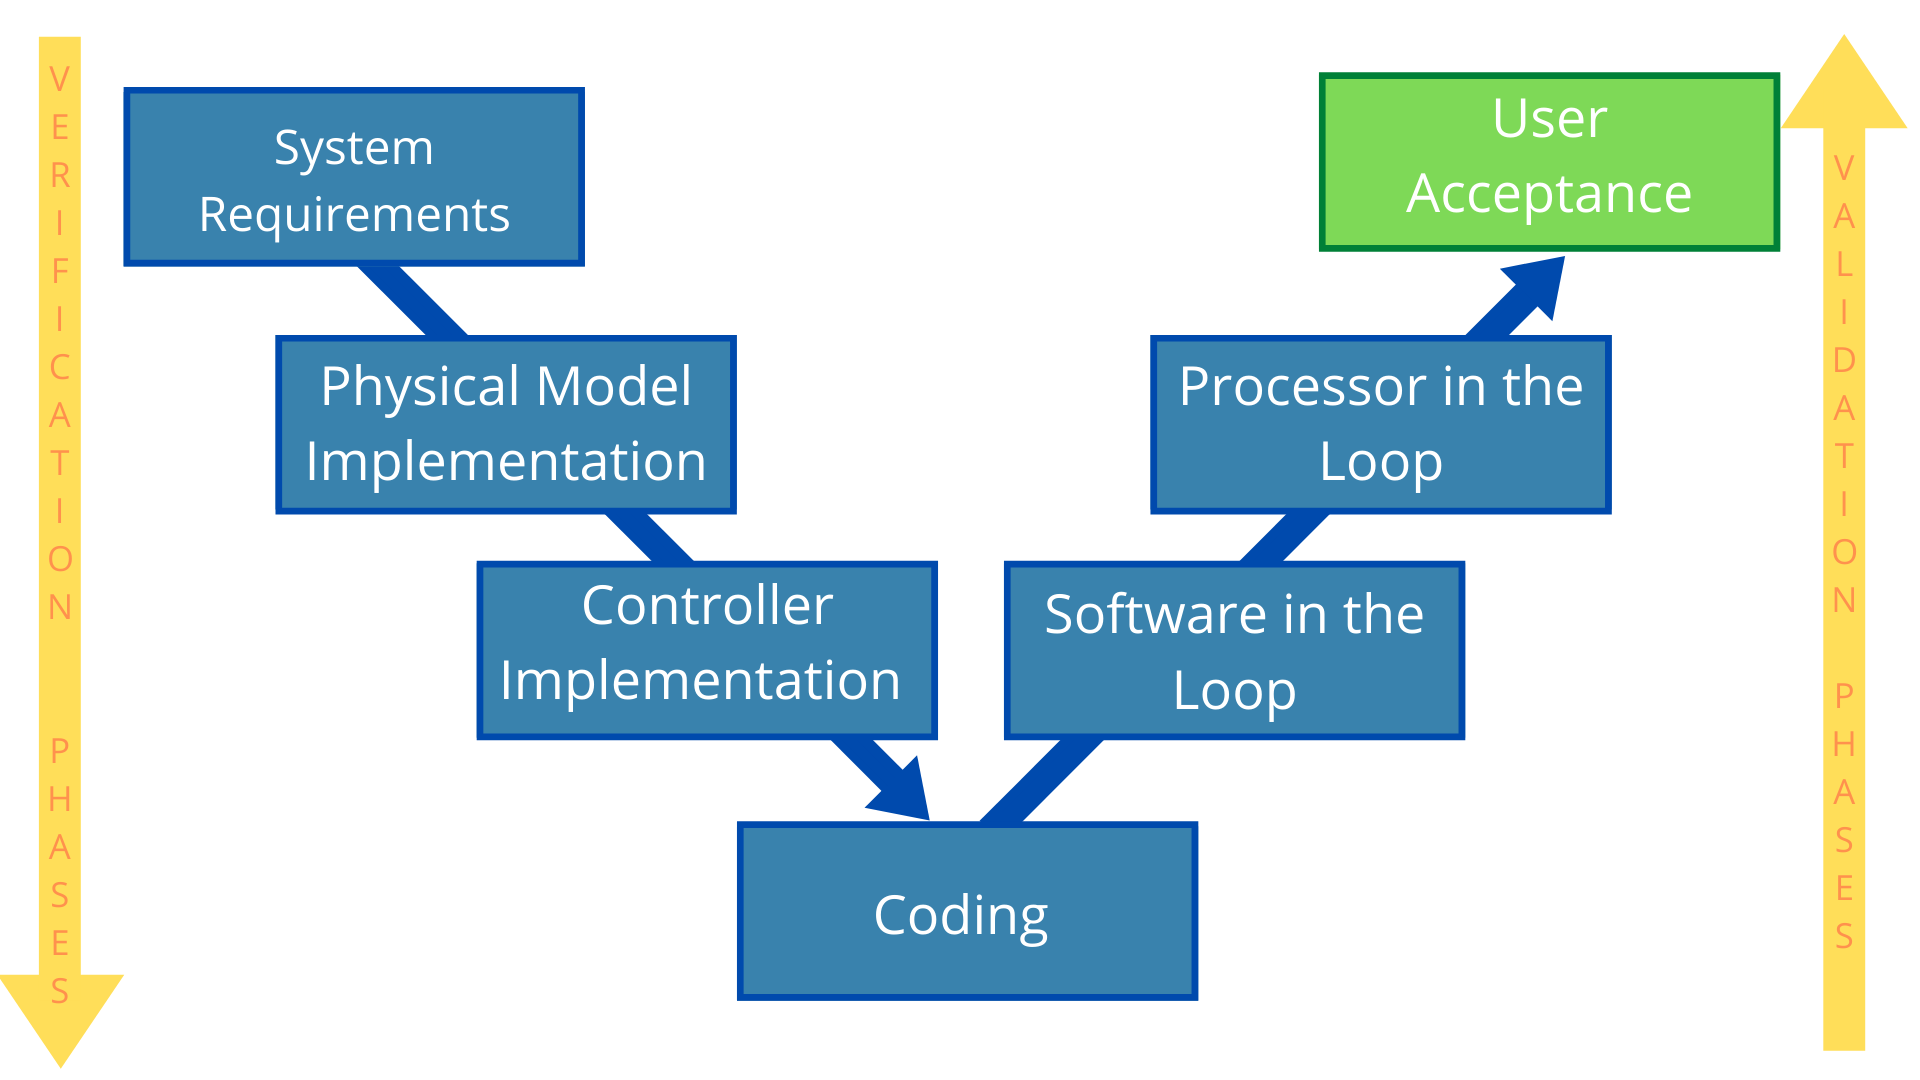
\includegraphics[width=1\textwidth]{Figures/V-MODEL.png}
    \caption{System Development V-model}
    
    \label{fig:V_model}
\end{figure}

As shown above the V-model is a representation of system development process that highlights verification steps on one side and validation steps on the other of the ‘V’. The left side of the ‘V’ identifies the verification phase, containing the steps that lead to code generation while the right side identifies the validation phase which ends with the user acceptance.
Below a brief description of the steps which constitute our V-model:
\begin{itemize}
    \item \textbf{System requirements}: this is the first step of each project, it consists in the requirements gathering from the customer;
    \item \textbf{Physical model implementation}: this phase contains the system design of our vehicle in terms of sensors required and dynamic and kinematic model;
    \item \textbf{Controller implementation}: this phase is the focus of our project, designing an adaptive MPC. 
    \item \textbf{Coding}: exploiting some specific tools, we can automatically generate code for embedded deployment and create test benches for system verification, saving time and avoiding the introduction of manually coded errors;
    \item \textbf{Software in the Loop}: once generated, the code is tested in a simulation environment;
    
    \item \textbf{Processor in the Loop}: during this phase the code is uploaded on a demo board and than it is tested again;
    
    \item \textbf{User Acceptance}: in this phase the final product is tested in order to verify the compliance with the initial costumer requirements.
\end{itemize}

\subsection{Required tools}
The project is based on \href{https://www.mathworks.com/help/matlab/index.html?s_tid=srchtitle}{\underline{MATLAB}}, a proprietary multi-paradigm programming language and numeric computing environment developed by \textit{MathWorks}, and \href{https://www.mathworks.com/help/simulink/index.html?s_tid=CRUX_lftnav}{\underline{Simulink}}, a MATLAB-based block diagram environment for multi-domain simulation and Model-Based Design.\\
The following list represents the software requirements for the project, including all the applications needed for the proper execution and test:
\begin{itemize}
    \item \textbf{MATLAB R2019a or newer};
    \begin{enumerate}
            \item \textbf{Curve Fitting Toolbox}: needed to make the reference map gentler;
            \item \textbf{Automated Driving Toolbox}: needed to get a reference map from real world data;
            \item \textbf{Model Predictive Control Toolbox}: needed to have all the useful resources to develop the MPC;
    \end{enumerate}
    \item \textbf{Simulink 9.3 or higher};
    \begin{enumerate}
            \item \textbf{Simulink Test}: used to perform automated tests and requirements verification;
            \item \textbf{Embedded Coder}: used for automatic code generation.
    \end{enumerate}
    
\end{itemize}




